\documentclass[12pt]{article}
\usepackage{ctex}
\usepackage{geometry}
\usepackage{amsmath}
\usepackage{graphicx}
\usepackage{listings}
\usepackage{xcolor}
\usepackage{longtable}

\title{核酸检测中的混检方案}
\author{第二十四届华东杯大学生数学建模邀请赛}
\date{2022.5}

\geometry{a4paper,left=2.5cm,right=2.5cm,top=2.5cm,bottom=2.5cm}

\definecolor{gray}{rgb}{0.99,0.99,0.99}

\lstdefinestyle{mystyle}{
basicstyle=\footnotesize,
backgroundcolor=\color{gray},
numbers=left
}

\lstset{style=mystyle}

\begin{document}

\maketitle

\begin{abstract}
这是一段摘要。这是一段摘要。这是一段摘要。这是一段摘要。这是一段摘要。这是一段摘要。这是一段摘要。这是一段摘要。这是一段摘要。这是一段摘要。这是一段摘要。这是一段摘要。这是一段摘要。这是一段摘要。这是一段摘要。这是一段摘要。这是一段摘要。这是一段摘要。这是一段摘要。这是一段摘要。
\end{abstract}

\newpage
\tableofcontents

\newpage
{\centering\section{问题的提出}}

2019年底、2020年初开始,新冠疫情席卷全球。
为了有效控制新冠病毒的传播,核酸检测是一个非常重要而有效的方法。
但是由于核酸检测需要一定的时间,在进行大规模检测时,往往会因为来不及检测而耽误控制病毒传播的宝贵时间。

为此,通常采用混合检测的方法。
将若干人组成一组,把他们的采样样本混合起来进行检测。
若一组核酸检测的结果为阴性,那么这组样本对应的被检测者都是阴性的。
若一组核酸检测的结果为阳性,那么这组样本对应的被检测者中至少有一人是阳性的,需要对这组样本的所有被检测者重新进行单人单管检测。

本文旨在回答以下几个问题:

1.单轮检测中,理想的混检方案;

2.根据现实数据,分析问题1.

3.多轮检测中,混检方案相对于单轮检测的调整。

{\centering\section{问题的初步分析}}

本文将由浅入深地建立两个模型:单轮检测模型和多轮检测模型。

定义一轮检测包括如下两个步骤:
先将若干人组成一组,进行混合检测;
若一组核酸检测的结果为阳性,
再对这组样本的所有被检测者进行单人单管检测。

在单轮检测模型中,仅进行一轮检测,
不考虑在核酸检测结果发布前的新增病例以及核酸检测本身的假阴性情况。
对于给定的总人口数和初始感染人数,
确定混合检测每组的人数,
使得核酸检测的总次数最小。

在多轮检测模型中,考虑进行多轮检测,
且考虑在核酸检测结果发布前的新增病例以及核酸检测本身的假阴性情况。
对于给定的总人口数、初始感染人数、传染系数、假阴性概率,
确定混合检测每组的人数、检测的次数、检测的间隔时间,
使得核酸检测的总次数尽可能小、人群中剩余病毒携带者的概率尽可能低。

\newpage
{\centering\section{单轮检测模型}}

\subsection{模型的假设}

1.仅进行一轮检测;

2.病毒携带者等可能地出现在各组中;

3.总人口数为常数;

4.不考虑在核酸检测结果发布前的新增病例,即感染病毒的人口数为常数;

5.不考虑核酸检测本身的假阴性情况;

6.核酸检测技术可以满足任意大的混合检测每组的人数。

\subsection{符号的说明}

\begin{table}[h]
\centering
\begin{tabular}{|l|l|} 
\hline
符号 & 含义 \\
\hline
$n$ & 总人口数 \\
$m$ & 感染病毒的人口数 \\
$k$ & 混合检测每组的人数 \\
\hline
\end{tabular}
\caption{单轮检测模型的符号说明}
\end{table}

\subsection{模型的建立}

记随机变量$X$表示单个人的核酸检测次数。
由于假设总人口数为常数,
最小化核酸检测的总次数即最小化单个人的核酸检测次数,
即最小化$E[X]$。

又由于假设病毒携带者等可能地出现在各组中,
$n$为总人口数,$m$为感染病毒的人口数,
可知任意一个人为病毒携带者的概率为$\frac{m}{n}$,
任意一组核酸检测为阴性的概率为$(1 - \frac{m}{n})^k$。
进而得到$X$的分布:
\begin{align*}
P(X = \frac{1}{k}) &= (1 - \frac{m}{n})^k \\
P(X = \frac{1}{k} + 1) &= 1 - (1 - \frac{m}{n})^k
\end{align*}

以及$X$的期望:
\begin{equation*}
E[X]
= \frac{1}{k} (1 - \frac{m}{n})^k + 
(\frac{1}{k} + 1)(1 - (1 - \frac{m}{n})^k)
= 1 + \frac{1}{k} - (1 - \frac{m}{n})^k
\end{equation*}

需要最小化上式。
特别地,当$ m \ll n $时,有
\begin{equation*}
E[X] \approx 1 + \frac{1}{k} - (1 - k\frac{m}{n})
= \frac{1}{k} + k\frac{m}{n}
\end{equation*}

当$ k = \sqrt{\frac{n}{m}} $时,
取得最小值$2\sqrt{\frac{m}{n}}$,
此时总核酸检测次数为$2\sqrt{mn}$,
且感染病毒的人口比例越高,单个人的核酸检测次数越高,符合预期。

\subsection{模型的应用}

本节将上述模型应用于上海市和吉林省长春市的新冠疫情情况。

根据上海市健康卫生委员会的疫情通报$^{[1]}$,
最近一轮的上海疫情始于2022年3月1日,每日新增一万左右例感染者。
再加上近期上海约两天进行一次核酸检测,可设置感染病毒的人口数为两万。

根据长春市健康卫生委员会的疫情通报$^{[2]}$,
最近一轮的长春疫情始于2022年3月5日,每日新增一千左右例感染者。
再加上近期长春约两天进行一次核酸检测$^{[3]}$,
可设置感染病毒的人口数为两千。

进而得到参数设置与实验结果如下:

\begin{table}[h]
\centering
\begin{tabular}{|c|c|c|c|c|c|c|c|} 
\hline
城市 & $n$ & $m$ & $ m / n $ & 
最优$k$ & 最优$E[X]$ & 
实际$k$ & 实际$E[X]$ \\
\hline
上海 & $ 2.4 \times 10^7 $ 
& $ 2 \times 10^4 $ & $ 8.3 \times 10^{-4} $ 
& 35 & 0.0573 
&  &  \\
长春 & $ 0.9 \times 10^7 $
& $ 2 \times 10^3 $ & $ 2.2 \times 10^{-4} $ 
& 68 & 0.0297 
&  &  \\
\hline
\end{tabular}
\caption{单轮检测模型应用的参数设置和实验结果}
\end{table}

\begin{figure}[h]
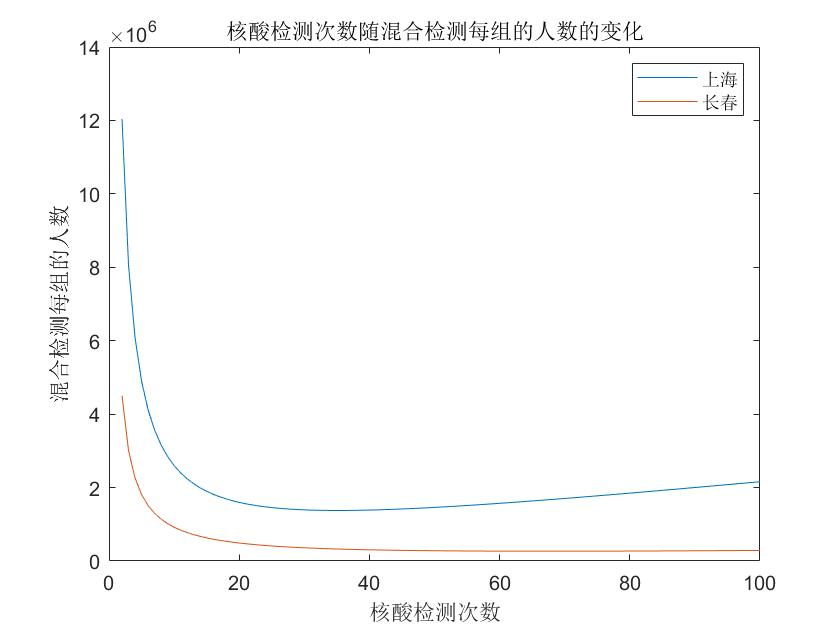
\includegraphics[width=\textwidth]{simple.jpg}
\caption{单轮检测模型应用的实验结果}
\end{figure}

\newpage
{\centering\section{多轮检测模型}}

\subsection{问题的分析}

在单轮检测模型中,
不考虑在核酸检测结果发布前的新增病例以及核酸检测本身的假阴性情况。
但事实上,上述两种情况都有可能发生,
使得核酸检测后人群中仍有可能剩余病毒携带者,
需要通过更多轮核酸检测检出。

因此,现建立多轮检测模型,
除了确定混合检测每组的人数,
还要确定检测的次数和间隔时间。

\subsection{模型的假设}

1.病毒携带者等可能地出现在各组中;

2.总人口数为常数;

3.不考虑被隔离人群传播病毒的能力;

4.核酸检测技术可以满足任意大的混合检测每组的人数。

\subsection{符号的说明}

\begin{table}[h]
\centering
\begin{tabular}{|l|l|} 
\hline
符号 & 含义 \\
\hline
$n$ & 总人口数 \\
$m$ & 最初感染病毒的人口数 \\
$\mu$ & 假阴性概率 \\
$\nu$ & 假阳性概率 \\
$\lambda$ & 一个病毒感染者单位时间将病毒传播给其他人的平均数量 \\
$\theta$ & 一个病毒感染者单位时间的治愈概率 \\
$QI$ & 当前感染病毒且被隔离的人数 \\
$QS$ & 当前未感染病毒但被隔离的人数 \\
$NS$ & 当前未感染病毒且未被隔离的人数 \\
$NI$ & 当前感染病毒但未被隔离的人数 \\
$k$ & 混合检测每组的人数 \\
\hline
\end{tabular}
\caption{多轮检测模型的符号说明}
\end{table}

\subsection{模型的建立}

\subsection{模型的应用}

{\centering\section{模型的评价与推广}}

\subsection{模型的评价}

\subsubsection{优点}

\subsubsection{缺点}

\subsection{模型的推广}

{\centering\section*{参考文献}}

[1]上海市卫生健康委员会,疫情通报,
https://wsjkw.sh.gov.cn/yqtb/,2022年5月1日。

[2]长春市卫生健康委员会,疫情通报,http://wjw.changchun.gov.cn/xwzx/tzgg/,2022年5月1日。

[3]长春e健康,长春市召开新型冠状病毒肺炎疫情防控工作第27场新闻发布会,https://mp.weixin.qq.com/s/V9W9oT-4coe\_LAABoooq5g,2022年5月2日。

\newpage
\appendix
{\centering\section*{附录}}

\section{数据}

\subsection{上海市疫情数据}

\begin{longtable}[c]{|c|r|r|r|r|}
\hline
日期 & 新增确诊 & 新增无症状 & 无症状转确诊 & 新增感病者 \\
\hline
3月1日 & 1 & 1 & 0 & 2 \\
3月2日 & 3 & 5 & 0 & 8 \\
3月3日 & 2 & 14 & 0 & 16 \\
3月4日 & 3 & 16 & 0 & 19 \\
3月5日 & 0 & 28 & 0 & 28 \\
3月6日 & 3 & 45 & 0 & 48 \\
3月7日 & 4 & 51 & 0 & 55 \\
3月8日 & 3 & 62 & 0 & 65 \\
3月9日 & 4 & 76 & 0 & 80 \\
3月10日 & 11 & 64 & 0 & 75 \\
3月11日 & 5 & 78 & 0 & 83 \\
3月12日 & 1 & 64 & 0 & 65 \\
3月13日 & 41 & 128 & 2 & 167 \\
3月14日 & 9 & 130 & 0 & 139 \\
3月15日 & 5 & 197 & 0 & 202 \\
3月16日 & 8 & 150 & 1 & 157 \\
3月17日 & 57 & 203 & 0 & 260 \\
3月18日 & 8 & 366 & 0 & 374 \\
3月19日 & 17 & 492 & 6 & 503 \\
3月20日 & 24 & 734 & 0 & 758 \\
3月21日 & 31 & 865 & 0 & 896 \\
3月22日 & 4 & 977 & 0 & 981 \\
3月23日 & 4 & 979 & 0 & 983 \\
3月24日 & 29 & 1580 & 0 & 1609 \\
3月25日 & 38 & 2231 & 5 & 2264 \\
3月26日 & 45 & 2631 & 0 & 2676 \\
3月27日 & 50 & 3450 & 0 & 3500 \\
3月28日 & 96 & 4381 & 21 & 4456 \\
3月29日 & 326 & 5656 & 18 & 5964 \\
3月30日 & 355 & 5298 & 16 & 5637 \\
\hline
日期 & 新增确诊 & 新增无症状 & 无症状转确诊 & 新增感病者 \\
\hline
3月31日 & 358 & 4144 & 20 & 4482 \\
4月1日 & 260 & 6051 & 2 & 6309 \\
4月2日 & 438 & 7788 & 73 & 8153 \\
4月3日 & 425 & 8581 & 71 & 8935 \\
4月4日 & 268 & 13086 & 4 & 13350 \\
4月5日 & 311 & 16766 & 40 & 17037 \\
4月6日 & 322 & 19660 & 15 & 19967 \\
4月7日 & 824 & 20398 & 323 & 20899 \\
4月8日 & 1015 & 22609 & 420 & 23204 \\
4月9日 & 1006 & 23937 & 191 & 24752 \\
4月10日 & 914 & 25173 & 47 & 26040 \\
4月11日 & 994 & 22348 & 273 & 23069 \\
4月12日 & 1189 & 25141 & 23 & 26307 \\
4月13日 & 2573 & 25146 & 114 & 27605 \\
4月14日 & 3200 & 19872 & 307 & 22765 \\
4月15日 & 3590 & 19923 & 922 & 22591 \\
4月16日 & 3238 & 21582 & 1177 & 23643 \\
4月17日 & 2471 & 19831 & 853 & 21449 \\
4月18日 & 3084 & 17332 & 974 & 19442 \\
4月19日 & 2494 & 16407 & 533 & 18368 \\
4月20日 & 2634 & 15861 & 459 & 18036 \\
4月21日 & 1931 & 15698 & 143 & 17486 \\
4月22日 & 2736 & 20634 & 1120 & 22250 \\
4月23日 & 1401 & 19657 & 541 & 20517 \\
4月24日 & 2472 & 16983 & 846 & 18609 \\
4月25日 & 1661 & 15319 & 968 & 16012 \\
4月26日 & 1606 & 11956 & 1253 & 12309 \\
4月27日 & 1292 & 9330 & 858 & 9764 \\
4月28日 & 5487 & 9545 & 5062 & 9970 \\
4月29日 & 1249 & 8932 & 85 & 9196 \\
4月30日 & 788 & 7084 & 683 & 7189 \\
\hline
\end{longtable}

\subsection{吉林省长春市疫情数据}

\begin{longtable}[c]{|l|r|r|r|r|}
\hline
日期 & 新增确诊 & 新增无症状 & 无症状转确诊 & 新增感病者 \\
\hline
3月5日 & 7 & 0 & 0 & 7 \\
\hline
日期 & 新增确诊 & 新增无症状 & 无症状转确诊 & 新增感病者 \\
\hline
3月6日 & 7 & 5 & 0 & 12 \\
3月7日 & 17 & 6 & 0 & 23 \\
3月8日 & 12 & 10 & 0 & 22 \\
3月9日 & 23 & 25 & 0 & 48 \\
3月10日 & 2 & 21 & 0 & 23 \\
3月11日 & 63 & 97 & 0 & 160 \\
3月12日 & 831 & 42 & 0 & 873 \\
3月13日 & 430 & 3 & 22 & 411 \\
3月14日 & 460 & 3 & 1 & 462 \\
3月15日 & 314 & 3 & 3 & 314 \\
3月16日 & 268 & 5 & 0 & 273 \\
3月17日 & 595 & 0 & 0 & 595 \\
3月18日 & 743 & 1 & 1 & 743 \\
3月19日 & 833 & 3 & 0 & 836 \\
3月20日 & 1079 & 1 & 2 & 1078 \\
3月21日 & 1437 & 0 & 2 & 1435 \\
3月22日 & 1979 & 0 & 57 & 1922 \\
3月23日 & 1280 & 253 & 0 & 1533 \\
3月24日 & 576 & 290 & 68 & 798 \\
3月25日 & 554 & 403 & 7 & 950 \\
3月26日 & 633 & 495 & 56 & 1072 \\
3月27日 & 706 & 330 & 120 & 916 \\
3月28日 & 622 & 310 & 11 & 921 \\
3月29日 & 875 & 348 & 19 & 1204 \\
3月30日 & 997 & 422 & 14 & 1405 \\
3月31日 & 1078 & 444 & 21 & 1501 \\
4月1日 & 1544 & 894 & 19 & 2419 \\
4月2日 & 723 & 3100 & 25 & 3798 \\
4月3日 & 574 & 2346 & 64 & 2856 \\
4月4日 & 604 & 1336 & 72 & 1868 \\
4月5日 & 817 & 1682 & 51 & 2448 \\
4月6日 & 766 & 1423 & 50 & 2139 \\
4月7日 & 474 & 1553 & 61 & 1966 \\
4月8日 & 150 & 648 & 50 & 748 \\
4月9日 & 175 & 703 & 90 & 788 \\
\hline
日期 & 新增确诊 & 新增无症状 & 无症状转确诊 & 新增感病者 \\
\hline
4月10日 & 102 & 743 & 29 & 816 \\
4月11日 & 81 & 570 & 28 & 623 \\
4月12日 & 173 & 801 & 96 & 878 \\
4月13日 & 285 & 621 & 212 & 694 \\
4月14日 & 138 & 298 & 79 & 357 \\
4月15日 & 157 & 407 & 57 & 507 \\
4月16日 & 125 & 491 & 33 & 583 \\
4月17日 & 144 & 348 & 41 & 451 \\
4月18日 & 74 & 365 & 26 & 413 \\
4月19日 & 125 & 243 & 69 & 299 \\
4月20日 & 88 & 233 & 32 & 289 \\
4月21日 & 53 & 21 & 25 & 49 \\
4月22日 & 129 & 188 & 83 & 234 \\
4月23日 & 45 & 127 & 16 & 156 \\
4月24日 & 74 & 89 & 39 & 124 \\
4月25日 & 34 & 89 & 19 & 104 \\
4月26日 & 46 & 66 & 31 & 81 \\
4月27日 & 52 & 89 & 27 & 114 \\
4月28日 & 34 & 39 & 28 & 45 \\
4月29日 & 19 & 29 & 12 & 36 \\
4月30日 & 16 & 23 & 11 & 28 \\
\hline
\end{longtable}

\newpage
\section{代码}

\subsection{单轮检测模型}

\begin{lstlisting}
clear;
clc;
close all;

% 上海
n = 2.4e7;
m = 2e4;

k = 2:100;
e = 1 + 1 ./ k - (1 - m / n) .^ k;
plot(k, n * e);
hold on;

% 长春
n = 9e6;
m = 2e3;

k = 2:100;
e = 1 + 1 ./ k - (1 - m / n) .^ k;
plot(k, n * e);

title('核酸检测次数随混合检测每组的人数的变化');
legend(['上海'; '长春'])
xlabel('核酸检测次数');
ylabel('混合检测每组的人数');
\end{lstlisting}


\end{document}